In this section, the effect of the code rate is investigated by fixing the constraint length. It has been chosen to fix the constraint length at $4$, and use codes with code rate $1/2$, $1/3$, and $1/4$, i.e. Code 4, Code 2 and Code 9, as specified in table \ref{tab:constraintLength}.
\\[6pt]
Figure \ref{fig:constantContraintRandomFigure} indicates that increasing the code rate greatly reduces the amount of errors in the BSC, as expected. Decreasing the code rate from $1/2$ to $1/3$ or from $1/3$ to $1/4$ reduces the BER by approximately an order of magnitude.
The effect on burst errors is also clear, as seen on figure \ref{fig:constantContraintBurstFigure}. Decreasing the code rate makes each burst cause less errors in the message. The same is seen in the MBEC, as shown on figure \ref{fig:constantContraintMarkovFigure}. The decrease of BER in this channel is much smaller than in the BSC, however.
In conclusion, the effect of varying the code rate is straightforward. More redundancy is added in the codeword causes less bit errors in the message, of course at the cost of decreasing the throughput in the channel.





%
%This section presents the results obtained by coding the messages with codes having the same constraint length (in our case, 4) but different code rates. All the three figures (figures \ref{fig:constantContraintRandomFigure}, \ref{fig:constantContraintRandomFigure}, \ref{fig:constantContraintMarkovFigure}) show the same result - the error correction capabilities are better when the code rate is lower. This is due to the fact that more redundancy is added to each message. As opposed to varying the constraint length, the variations in code rate have a straight forward result.

\begin{figure}
\centering
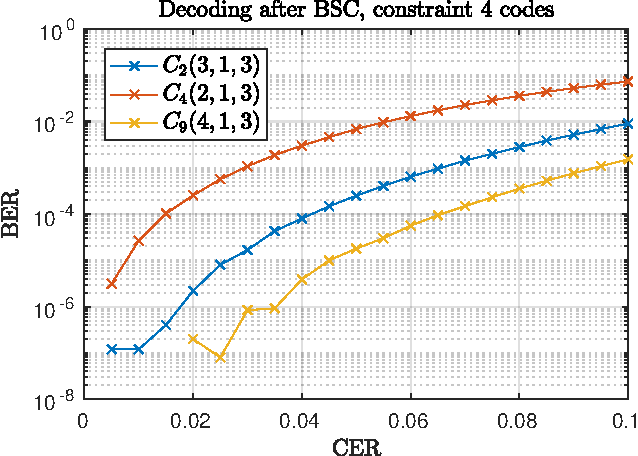
\includegraphics[scale=1]{../figures/const4rand.pdf} 
\caption{\textit{Comparison of codes with constraint length 4 and varying code rates in BSC}\label{fig:constantContraintRandomFigure}}
\end{figure}

\begin{figure}
\centering
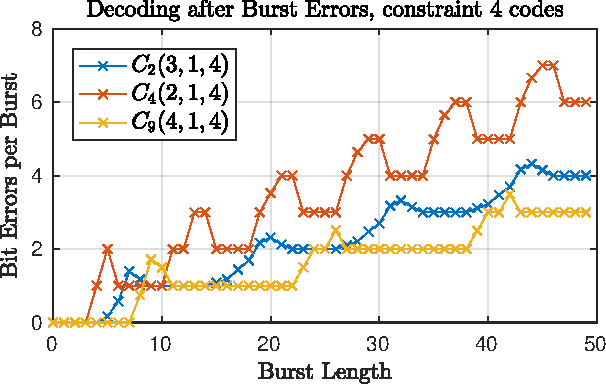
\includegraphics[scale=1]{../figures/const4burst.pdf} 
\caption{\textit{Comparison of codes with constraint length 4 and varying code rates burst correction capabilities}\label{fig:constantContraintBurstFigure}}	
\end{figure}

\begin{figure}
\centering
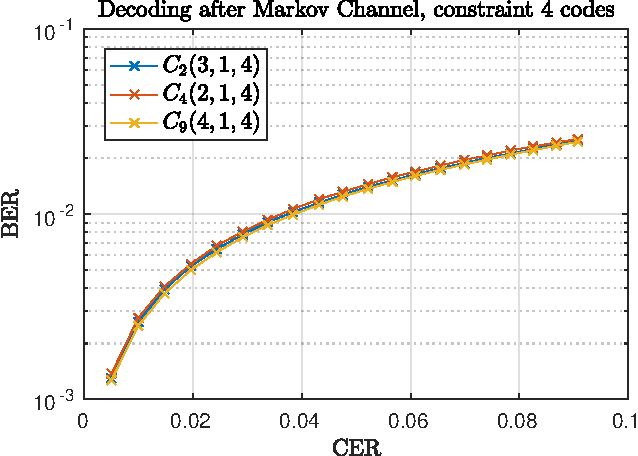
\includegraphics[scale=1]{../figures/const4markov.pdf} 
\caption{\textit{Comparison of codes with constraint length 4 and varying code rates in MBEC}\label{fig:constantContraintMarkovFigure}}
\end{figure}